\documentclass[11pt,letterpaper]{article}
\usepackage[T1]{fontenc}
\usepackage[scaled]{helvet}
\renewcommand{\familydefault}{\sfdefault}
\usepackage{amsmath,amssymb}
\usepackage[margin=0.8in,bottom=0.9in]{geometry}
\usepackage[most]{tcolorbox}
\usepackage{tikz}
\usetikzlibrary{calc}
\usepackage{enumitem}
\usepackage{array}
\usepackage{needspace}
\usepackage{fancyhdr}
\usepackage{pifont}

% ---- Palette "F. Bright & Playful" ----
\definecolor{fmtitle}{HTML}{3D2C8D}
\definecolor{fmkey}{HTML}{0096C7}
\definecolor{fmwatch}{HTML}{2BB673}
\definecolor{fmturn}{HTML}{F4A100}
\definecolor{fmmistake}{HTML}{EF476F}
\definecolor{fmnotice}{HTML}{9B5DE5}
\definecolor{fmgray}{HTML}{6B6B6B}

\pagestyle{fancy}
\fancyhf{}
\renewcommand{\headrulewidth}{0pt}
\fancyfoot[C]{\footnotesize\color{fmgray}\textcopyright\ 2026 FangMath. All rights reserved.}
\fancyfoot[R]{\footnotesize\color{fmgray}\thepage}
\setlength{\parindent}{0pt}
\setlength{\parskip}{3pt}

\newcommand{\badge}[1]{\colorbox{fmtitle}{\color{white}\bfseries\small\ #1\ }}
\newcommand{\leveltag}[2]{\colorbox{#1}{\color{white}\bfseries\scriptsize\ #2\ }}
\newcommand{\LE}{\leveltag{fmwatch}{EASY}}
\newcommand{\LM}{\leveltag{fmturn}{MEDIUM}}
\newcommand{\LH}{\leveltag{fmmistake}{HARD}}

\newcommand{\sectionbar}[2]{\needspace{6cm}\par\vspace{4mm}
  \begin{tcolorbox}[enhanced,colback=fmtitle,colframe=fmtitle,arc=2mm,
    left=4mm,top=1.5mm,bottom=1.5mm]
  \color{white}\bfseries\large #1\hfill{\normalsize\mdseries #2}
  \end{tcolorbox}}

\newtcolorbox{keyidea}{enhanced,breakable,colback=white,colframe=fmkey,boxrule=1pt,arc=2mm,
  title={Key Idea},coltitle=fmkey,fonttitle=\bfseries,
  attach boxed title to top left={xshift=4mm,yshift=-2mm},
  boxed title style={colback=white,colframe=fmkey,boxrule=0.9pt}}
\newtcolorbox{watchme}{enhanced,colback=white,colframe=fmwatch,boxrule=1pt,arc=2mm,
  title={Watch Me --- Worked Example},coltitle=fmwatch,fonttitle=\bfseries,
  attach boxed title to top left={xshift=4mm,yshift=-2mm},
  boxed title style={colback=white,colframe=fmwatch,boxrule=0.9pt}}
\newtcolorbox{mistakebox}{enhanced,breakable,colback=white,colframe=fmmistake,boxrule=1pt,arc=2mm,
  title={Common Mistake},coltitle=fmmistake,fonttitle=\bfseries,
  attach boxed title to top left={xshift=4mm,yshift=-2mm},
  boxed title style={colback=white,colframe=fmmistake,boxrule=0.9pt}}
\newtcolorbox{yourturn}{enhanced,breakable,colback=white,colframe=fmturn,boxrule=1pt,arc=2mm,
  title={Your Turn},coltitle=fmturn,fonttitle=\bfseries,
  attach boxed title to top left={xshift=4mm,yshift=-2mm},
  boxed title style={colback=white,colframe=fmturn,boxrule=0.9pt}}
\newtcolorbox{answerbox}[1]{enhanced,breakable,colback=white,colframe=fmwatch,boxrule=1pt,arc=2mm,
  title={#1},coltitle=fmwatch,fonttitle=\bfseries,
  attach boxed title to top left={xshift=4mm,yshift=-2mm},
  boxed title style={colback=white,colframe=fmwatch,boxrule=0.9pt}}

\newcommand{\work}[1]{\par\vspace{#1}}
\setlist[enumerate]{itemsep=2pt,topsep=3pt}

% ---------------- extra boxes ----------------
\newtcolorbox{notebox}{enhanced,breakable,colback=white,colframe=fmnotice,boxrule=1pt,arc=2mm,
  title={Notice},coltitle=fmnotice,fonttitle=\bfseries,
  attach boxed title to top left={xshift=4mm,yshift=-2mm},
  boxed title style={colback=white,colframe=fmnotice,boxrule=0.9pt}}
\newtcolorbox{exbox}{enhanced,colback=white,colframe=fmwatch,boxrule=0.8pt,arc=2mm,
  title={Example},coltitle=fmwatch,fonttitle=\bfseries\small,
  attach boxed title to top left={xshift=4mm,yshift=-2mm},
  boxed title style={colback=white,colframe=fmwatch,boxrule=0.8pt},fontupper=\small}
\newcommand{\topicbar}[1]{\needspace{4.5cm}\par\vspace{5mm}
  \begin{tcolorbox}[enhanced,colback=fmtitle,colframe=fmtitle,arc=2mm,left=4mm,top=1.5mm,bottom=1.5mm]
  \color{white}\bfseries\large #1
  \end{tcolorbox}}
\usepackage{multicol}

% ---------------- practice layout ----------------
\newcommand{\workline}{\par\vspace{7mm}{\color{gray!55}\rule{\linewidth}{0.4pt}}}
\newcommand{\worklines}[1]{\foreach \i in {1,...,#1}{\workline}}
\newcommand{\prob}[3]{\needspace{#3}\par\vspace{3mm}{\color{fmturn}\bfseries #1.}\ #2\par}
\newcommand{\ansline}{\par\vspace{4mm}\hfill\textbf{Answer:}\ \rule{5cm}{0.4pt}\par}
\newcommand{\keyitem}[3]{\needspace{3.2cm}\par\vspace{2mm}
  \begin{tcolorbox}[enhanced,colback=white,colframe=fmwatch!60,boxrule=0.6pt,arc=1.5mm,left=3mm,top=1.5mm,bottom=1.5mm]
  {\color{fmwatch}\bfseries #1.}\quad\small #2\par\vspace{1mm}
  \normalsize\textbf{Answer: #3}
  \end{tcolorbox}}


\usetikzlibrary{arrows.meta}
\providecommand{\iskey}{0}
% fill-in blank: line for students, pink answer in the key
\newcommand{\fb}[2][2.6cm]{\ifnum\iskey=1 \underline{\makebox[#1][c]{\color{fmmistake}\bfseries #2}}\else\underline{\makebox[#1]{}}\fi}
% answer line for practice problems
\newcommand{\pans}[2][3.2cm]{\ifnum\iskey=1 \underline{\makebox[#1][c]{\color{fmmistake}\bfseries #2}}\else\rule{#1}{0.4pt}\fi}
\newcommand{\vid}[1]{{\color{fmgray}\small\textit{\ding{43} Video: #1}}}
\newcommand{\pt}[2]{\fill (#1) circle (2.2pt) node[above=1pt,font=\small]{$#2$};}

\usetikzlibrary{decorations.pathreplacing}
\newcommand{\gridb}[4]{\draw[gray!30,step=1] (#1,#2) grid (#3,#4);\draw[gray!70,-{Stealth}] (#1,0)--(#3+0.4,0);\draw[gray!70,-{Stealth}] (0,#2)--(0,#4+0.4);}
\newcommand{\sdp}[3]{\begin{minipage}[t][2.4cm]{0.48\linewidth}{\color{fmturn}\bfseries #1.}\ #2\par\vfill\hfill \pans[3.6cm]{#3}\end{minipage}}
\newcommand{\sdpw}[3]{\begin{minipage}[t][2.4cm]{0.48\linewidth}{\color{fmturn}\bfseries #1.}\ #2\par\vfill\hfill \pans[5.2cm]{#3}\end{minipage}}
\newcommand{\algp}[3]{\begin{minipage}[t][4.2cm]{0.48\linewidth}{\color{fmturn}\bfseries #1.}\ #2\par\vfill\hfill \pans[4.4cm]{#3}\end{minipage}}
\newcommand{\pair}[2]{\needspace{3.4cm}\noindent #1\hfill #2\par\vspace{2mm}}
\newcommand{\head}[2]{\ifnum\iskey=1 \colorbox{fmwatch}{\color{white}\bfseries\small\ ANSWER KEY\ }\else\badge{#1}\fi\hfill{\small\color{fmgray}Geometry \textperiodcentered\ Lesson #2}\par\vspace{4mm}}
\newcommand{\nameline}{Name: \rule{6cm}{0.4pt}\hspace{1cm}Date: \rule{3.5cm}{0.4pt}\par\vspace{2mm}}
\renewcommand{\vid}[1]{\needspace{4.2cm}{\color{fmgray}\small\textit{\ding{43} Video: #1}}}
\newcommand{\cbox}[3]{\begin{minipage}[t][6.4cm]{0.48\linewidth}{\color{fmturn}\bfseries #1.}\ #2\par\vspace{2mm}\centering #3\end{minipage}}
\begin{document}
\head{PRACTICE}{1.6}
{\color{fmtitle}\LARGE\bfseries Constructions --- Practice\ifnum\iskey=1 \ --- Answer Key\fi}\par\vspace{1mm}
{\color{fmgray}You need a compass, a straightedge and a pencil. A worked example comes before each type.}\par\vspace{3mm}
\nameline

\needspace{6cm}\topicbar{Type 1 \quad Tools \& Words}
\begin{watchme}In a construction, may you use the inch marks on a ruler?\par
No --- a straightedge only draws straight lines. Lengths are copied with the compass. \quad \textbf{Answer: no}\end{watchme}
\pair{\sdp{1}{Which tool copies a length?}{compass}}{\sdp{2}{Which tool draws straight lines?}{straightedge}}
\pair{\sdp{3}{A bisector cuts a segment or an angle into two \underline{\hspace{1.5cm}} parts.}{equal}}{\sdpw{4}{The perpendicular bisector meets the segment at its \underline{\hspace{1.5cm}}, at a \underline{\hspace{1.5cm}} angle.}{midpoint,\ right ($90^\circ$)}}

\needspace{6cm}\topicbar{Type 2 \quad Choose the Compass Width}
\begin{watchme}To bisect a $10$ cm segment, how wide must the compass be?\par
More than half of $10$ cm, so more than $5$ cm (for example $6$ cm). \quad \textbf{Answer: more than 5 cm}\end{watchme}
\pair{\sdp{5}{A segment is $12$ cm. Which width works: $5$ cm or $7$ cm?}{$7$ cm}}{\sdp{6}{A segment is $9$ cm. What is the smallest whole-cm width that works?}{$5$ cm}}
\pair{\sdpw{7}{Why must both arcs use the \textbf{same} width?}{so $P$ and $Q$ are equally far from $A$ and $B$}}{\sdp{8}{On a number line $A$ is at $2$ and $B$ is at $14$. Where does the perpendicular bisector cross?}{at $8$}}

\needspace{8cm}\topicbar{Type 3 \quad Construct It}
\begin{watchme}Leave every arc on the page --- the arcs are your ``show your work.'' Check with a ruler only at the very end.\end{watchme}
\needspace{6.6cm}\noindent\cbox{9}{Bisect $\overline{AB}$ (it is $6$ cm). Label the midpoint $M$.}{\begin{tikzpicture}[scale=0.75,every node/.style={scale=1}]\draw[very thick] (0,0)--(6,0);\fill (0,0) circle(2pt) node[below left]{$A$} (6,0) circle(2pt) node[below right]{$B$};
\ifnum\iskey=1 \draw[fmkey,thick] (0,0) ++(32:4) arc (32:50:4);\draw[fmkey,thick] (0,0) ++(-32:4) arc (-32:-50:4);\draw[fmturn,thick] (6,0) ++(148:4) arc (148:130:4);\draw[fmturn,thick] (6,0) ++(-148:4) arc (-148:-130:4);
\draw[fmmistake,thick] (3,2.9)--(3,-2.9);\fill[fmmistake] (3,0) circle(2.2pt) node[below right]{$M$};\node[fmmistake,font=\small,anchor=west] at (3.35,-1.9){$AM = MB = 3$ cm};\else\path (0,-2.9) rectangle (6,2.9);\fi\end{tikzpicture}}\hfill
\cbox{10}{Bisect $\angle B$ (it is $70^\circ$).}{\begin{tikzpicture}\draw[very thick,-{Stealth}] (0,0)--(4.4,0);\draw[very thick,-{Stealth}] (0,0)--(70:4.2);\fill (0,0) circle(2pt) node[below left]{$B$};
\ifnum\iskey=1 \draw[fmkey,thick] (2,0) arc (0:70:2);\draw[fmturn,thick] (2,0) ++(66:1.6) arc (66:96:1.6);\draw[fmturn,thick] (70:2) ++(-25:1.6) arc (-25:4:1.6);
\draw[fmmistake,thick,-{Stealth}] (0,0)--(35:4.4);\node[fmmistake,font=\small] at (2.3,-0.5){two $35^\circ$ angles};\else\path (0,-0.6) rectangle (4.4,4);\fi\end{tikzpicture}}\par\vspace{2mm}
\needspace{6.6cm}\noindent\cbox{11}{Copy $\overline{AB}$ onto the ray, starting at $C$. Label the new endpoint $D$.}{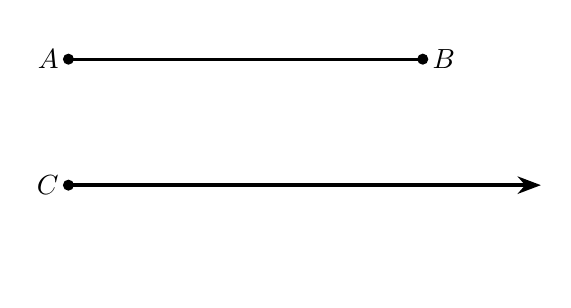
\begin{tikzpicture}\draw[very thick] (0,1.6)--(4.5,1.6);\fill (0,1.6) circle(2pt) node[left]{$A$} (4.5,1.6) circle(2pt) node[right]{$B$};
\draw[very thick,-{Stealth}] (0,0)--(6,0);\fill (0,0) circle(2pt) node[left]{$C$};
\ifnum\iskey=1 \draw[fmkey,thick] (0,0) ++(-12:4.5) arc (-12:12:4.5);\fill[fmmistake] (4.5,0) circle(2.2pt) node[below]{$D$};\node[fmmistake,font=\small] at (3,-0.9){$CD = AB$};\fi\path (0,-1.2) rectangle (6,2);\end{tikzpicture}}\hfill
\cbox{12}{\LH\ Bisect the right angle to make a $45^\circ$ angle.}{\begin{tikzpicture}\draw[very thick,-{Stealth}] (0,0)--(4,0);\draw[very thick,-{Stealth}] (0,0)--(0,4);\draw (0.3,0)--(0.3,0.3)--(0,0.3);\fill (0,0) circle(2pt);
\ifnum\iskey=1 \draw[fmkey,thick] (2,0) arc (0:90:2);\draw[fmturn,thick] (2,0) ++(80:2) arc (80:100:2);\draw[fmturn,thick] (0,2) ++(-10:2) arc (-10:10:2);
\draw[fmmistake,thick,-{Stealth}] (0,0)--(45:4.3);\node[fmmistake,font=\small] at (3.1,1.2){$45^\circ$};\fi\path (0,0) rectangle (4,4);\end{tikzpicture}}\par

\needspace{6.5cm}\topicbar{Type 4 \quad Use What a Bisector Does}
\begin{watchme}$M$ is the midpoint of $\overline{AB}$. $AM = 2x + 3$ and $MB = 4x - 5$. Find $AB$.\par
A midpoint makes equal halves: $2x + 3 = 4x - 5$, so $x = 4$. Each half is $11$, so $AB = 22$. \quad \textbf{Answer: $\boldsymbol{22}$}\end{watchme}
\pair{\sdp{13}{An $84^\circ$ angle is bisected. How big is each half?}{$42^\circ$}}{\sdp{14}{$M$ is the midpoint of $\overline{AB}$. $AM = 3x + 1$, $MB = 5x - 7$. Find $AB$.}{$AB = 26$}}
\pair{\sdpw{15}{$\overrightarrow{BZ}$ bisects $\angle ABC$. $m\angle ABZ = 2x + 10$, $m\angle ZBC = 4x - 6$. Find $m\angle ABC$.}{$x = 8,\ 52^\circ$}}{\sdpw{16}{Why is the crossing point $P$ the same distance from $A$ and from $B$?}{both arcs have the same radius}}
\end{document}
